\documentclass[conference,a4paper]{IEEEtran}

% Packages
\usepackage{cite}
\usepackage{amsmath,amssymb,amsfonts}
\usepackage{algorithmic}
\usepackage{graphicx}
\usepackage{textcomp}
\usepackage{xcolor}
\usepackage{booktabs}
\usepackage{multirow}
\usepackage[hidelinks]{hyperref}
\usepackage{float}
\usepackage{array}
\usepackage{caption}
\usepackage{subcaption}
\usepackage{tikz}
\usetikzlibrary{positioning, arrows.meta, calc}

\def\BibTeX{{\rm B\kern-.05em{\sc i\kern-.025em b}\kern-.08em
    T\kern-.1667em\lower.7ex\hbox{E}\kern-.125emX}}

\begin{document}

\title{Object Classification Using Ultrasonic Pulse-Echo Signals: A Comparative Study of Classical Machine Learning and Deep Learning Approaches}

\author{
\IEEEauthorblockA{Information Technology\\Machine Learning 2025\\Fahim Talukdar\\Mat: 1428610\\
fahim.talukdar@stud.fra-uas.de}
\and
\IEEEauthorblockA{Information Technology\\Machine Learning 2025\\Md Ashraf Uddin\\Mat: 1398481\\
ashraf.uddin@stud.fra-uas.de}
\and
\IEEEauthorblockA{Information Technology\\Machine Learning 2025\\Md Tanzeem Hasan Mahmud\\Mat: 1364198\\
mahmud.mdtanzeemhasan@stud.fra-uas.de}
}

\maketitle

% ==============================================================
% ABSTRACT
% ==============================================================
\begin{abstract}
This paper investigates whether ultrasonic pulse-echo signals carry enough information to reliably distinguish between a human body, an office chair, and an empty floor. Using a FIUS smart sensor operating at 40\,kHz with a sampling rate of 1,953,125\,S/s, we collected 15,007 echo measurements across three classes and explored two classification strategies in parallel. The first strategy relied on 52 handcrafted features---spanning segmented energy, peak timing, and spectral characteristics---fed into six classical machine learning models. XGBoost led this group with 99.97\% test accuracy. The second strategy bypassed feature engineering entirely, feeding raw downsampled signals into three deep learning architectures: a 1D-CNN (99.33\%), a 1D-ResNet (99.20\%), and a 1D-Transformer (99.53\%). We validated these results through temporal cross-validation, learning curve analysis, noise injection, and label-shuffling tests to rule out overfitting. Finally, the deep learning models were deployed in a real-time PyQt6 application connected to the sensor via UDP, where a majority-vote consensus across all three networks provided robust live classification. The results confirm that material-dependent differences in ultrasonic echo patterns offer a reliable basis for object classification, with both classical and deep learning methods comfortably exceeding a 95\% accuracy threshold.
\end{abstract}

\begin{IEEEkeywords}
ultrasonic sensor, object classification, machine learning, deep learning, 1D-CNN, Transformer, ResNet, pulse-echo, signal classification, real-time inference
\end{IEEEkeywords}

% ==============================================================
% I. INTRODUCTION
% ==============================================================
\section{Introduction}

Ultrasonic sensors have long served as workhorses for non-contact distance measurement in industrial automation, robotics, and building management systems \cite{carullo2001}. A typical ultrasonic system emits a short acoustic pulse and measures the time until the echo returns, yielding a distance estimate. What these systems generally do \emph{not} provide is any characterization of the reflecting object itself. In many practical settings---smart offices that need to distinguish an occupied desk from an empty one, autonomous robots navigating cluttered rooms, or access-control systems---knowing \emph{what} is present matters as much as knowing \emph{how far away} it is.

The underlying physics suggests that classification should be feasible. A soft, irregular body like a human absorbs and scatters ultrasonic waves in a pattern quite different from a hard, flat surface like a chair seat, which in turn differs from the unobstructed floor. Each of these interactions leaves a distinctive fingerprint in the time-domain echo signal. The question is whether machine learning can exploit these fingerprints reliably.

This paper addresses that question for a three-class problem---Human, Chair, and Nothing (empty floor)---using data from a custom FIUS smart ultrasonic sensor. We pursue two parallel approaches. In the first, we design a pipeline of 52 handcrafted signal features and benchmark six well-known classifiers (Random Forest, XGBoost, LightGBM, SVM, KNN, and Logistic Regression). In the second, we feed the raw echo waveform directly into three neural network architectures---a standard 1D-CNN, a deeper 1D-ResNet with skip connections, and a 1D-Transformer with self-attention---and let the networks discover their own representations. We then validate all models against overfitting through four independent tests and deploy the best-performing networks for live inference on the physical sensor.

The paper proceeds as follows. Section~II describes the sensor hardware and the data collection protocol. Section~III lays out the feature engineering pipeline and the model architectures. Section~IV presents the experimental results, including offline accuracy, overfitting validation, and real-time deployment. Section~V discusses the trade-offs between classical and deep learning approaches, and Section~VI concludes.

% ==============================================================
% II. SENSOR AND DATA ACQUISITION
% ==============================================================
\section{Sensor and Data Acquisition}

\subsection{FIUS Ultrasonic Sensor}

The FIUS smart sensor is built around a 40\,kHz piezoelectric transducer operated in pulse-echo mode. After emitting a short burst, the sensor records the returning echo through a 14-bit analog-to-digital converter (ADC) running at 1,953,125\,S/s---roughly 1.95 million samples per second. Each acquisition captures 25,000 consecutive samples, covering a time window of approximately 12.8\,ms. At the speed of sound in air ($c \approx 343.2$\,m/s), this corresponds to a maximum round-trip path of about 2.20\,m, or an effective one-way detection range of roughly 1.10\,m.

The analog front-end and digitizer sit on a Red Pitaya FPGA development board, which handles the high-speed acquisition and streams the data over UDP to a host PC. Each UDP packet carries 17 floating-point metadata values---including sensor configuration parameters, a firmware-computed distance estimate, and a signal energy metric---followed by the 25,000 raw ADC samples.

\subsection{Data Collection}

We mounted the sensor vertically on a fixed stand, pointing straight down toward the floor, and collected data for three target classes:

\begin{itemize}
    \item \textbf{Human}: A person standing, sitting, or moving beneath the sensor. We deliberately varied the posture across recording sessions to ensure that the dataset captures the natural variability of soft-body reflections.
    \item \textbf{Chair}: A standard office swivel chair positioned under the sensor, representing a hard, geometrically regular reflector.
    \item \textbf{Nothing}: The bare floor with no object in the sensor's field of view, producing only a floor-level return at the maximum detectable range.
\end{itemize}

Roughly 5{,}000 measurements were recorded per class, yielding a balanced corpus of 15{,}007 samples in total. Each sample was stored as a single CSV row containing the 17 metadata fields followed by the 25{,}000 signal values. No samples contained missing or corrupted entries.

\subsection{Signal Characteristics}

Visual inspection of the averaged echo waveforms immediately reveals that the three classes produce qualitatively different signals, as shown in Fig.~\ref{fig:mean_signals}. The Human signal is characterized by low-amplitude, diffuse reflections spread across the recording window, with a slight concentration in the first 1--3\,ms. The Chair signal is dominated by a sharp, high-amplitude burst around 6\,ms, consistent with specular reflection from a hard surface at a known distance. The Nothing signal is nearly silent except for a pronounced spike near 10.5\,ms, which corresponds to the floor echo.

\begin{figure}[H]
\centering
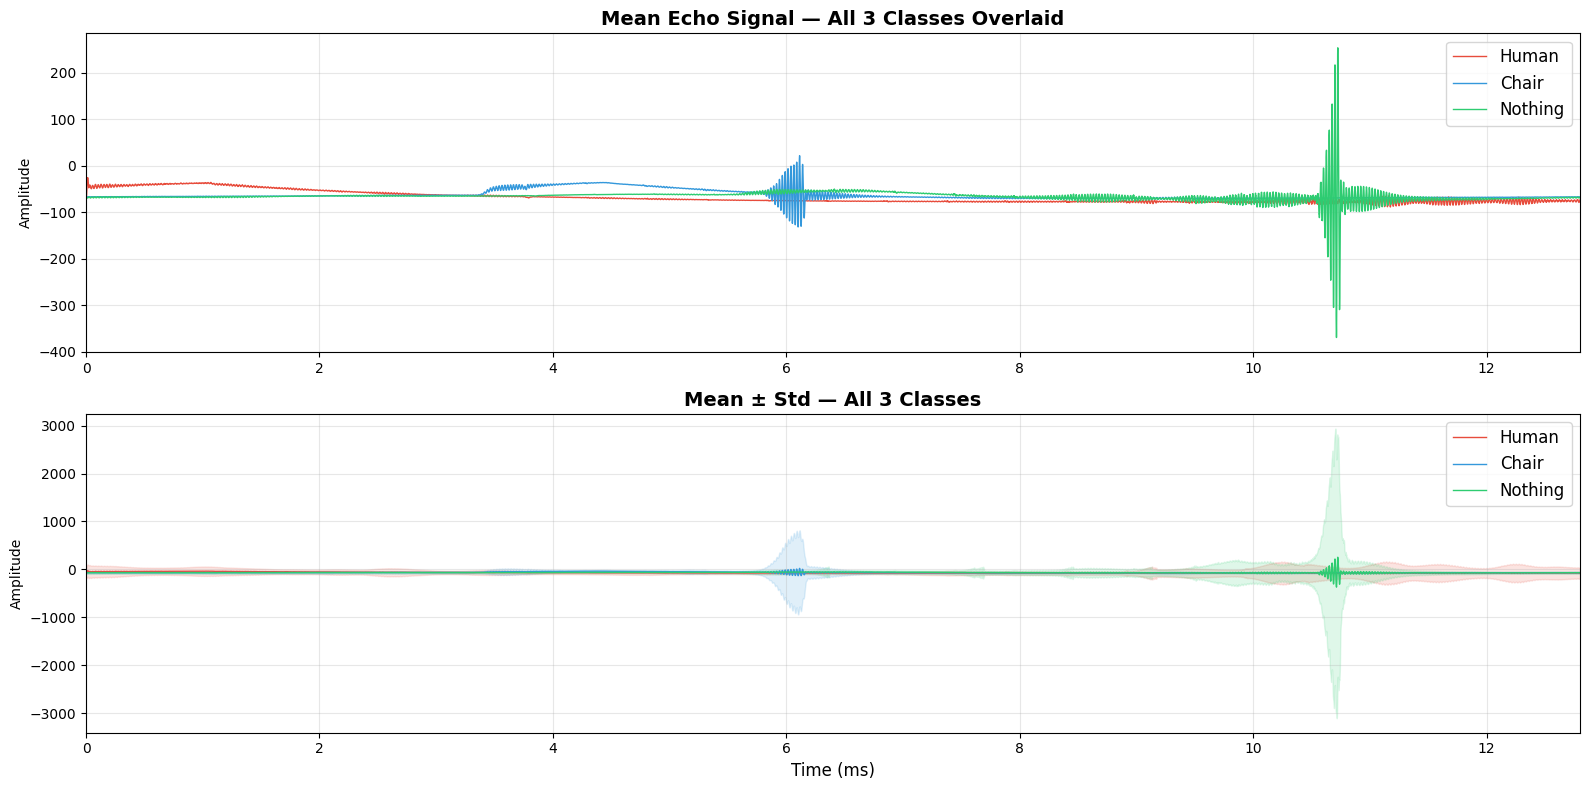
\includegraphics[width=\columnwidth]{fig_mean_signals.png}
\caption{Averaged echo waveforms for the three classes. Top panel: mean signal; bottom panel: mean $\pm$ one standard deviation. Human echoes are weak and distributed, Chair echoes are sharp and localized around 6\,ms, and Nothing echoes consist mainly of a floor reflection near 10.5\,ms.}
\label{fig:mean_signals}
\end{figure}

To quantify these differences, we divided each signal into 25 non-overlapping windows of 1{,}000 samples ($\approx$0.51\,ms each) and computed the mean energy per window for each class (Fig.~\ref{fig:segmented_energy}). The resulting energy profiles are strikingly distinct: Nothing concentrates nearly all its energy in a single late-time window, Chair peaks in the mid-range, and Human distributes energy more broadly. This segmented energy profile turns out to be the single most informative representation for classification, as the feature importance analysis in Section~IV-B will confirm.

\begin{figure}[H]
\centering
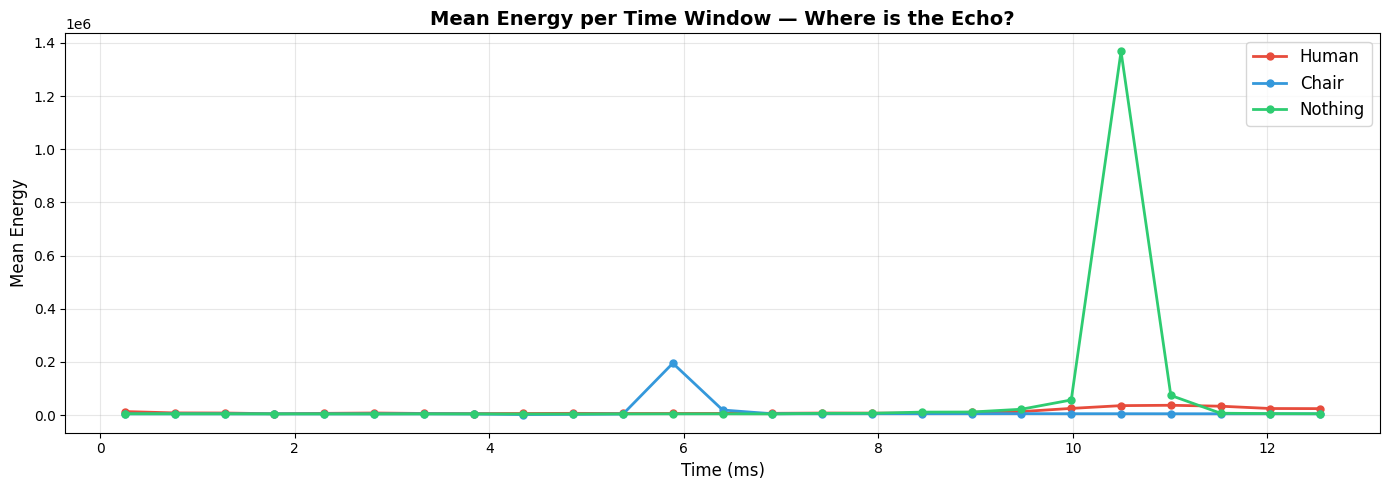
\includegraphics[width=\columnwidth]{fig_segmented_energy.png}
\caption{Mean energy per time window for each class. The 25,000-sample signal is divided into 25 windows of 1,000 samples each. The three classes concentrate their echo energy in clearly separated temporal regions, providing a strong discriminative basis.}
\label{fig:segmented_energy}
\end{figure}

% ==============================================================
% III. METHODOLOGY
% ==============================================================
\section{Methodology}

We explored two complementary classification strategies: one based on handcrafted features with classical ML, and one based on raw signal input with deep learning.
\begin{figure}[H]
\centering
\resizebox{\columnwidth}{!}{%
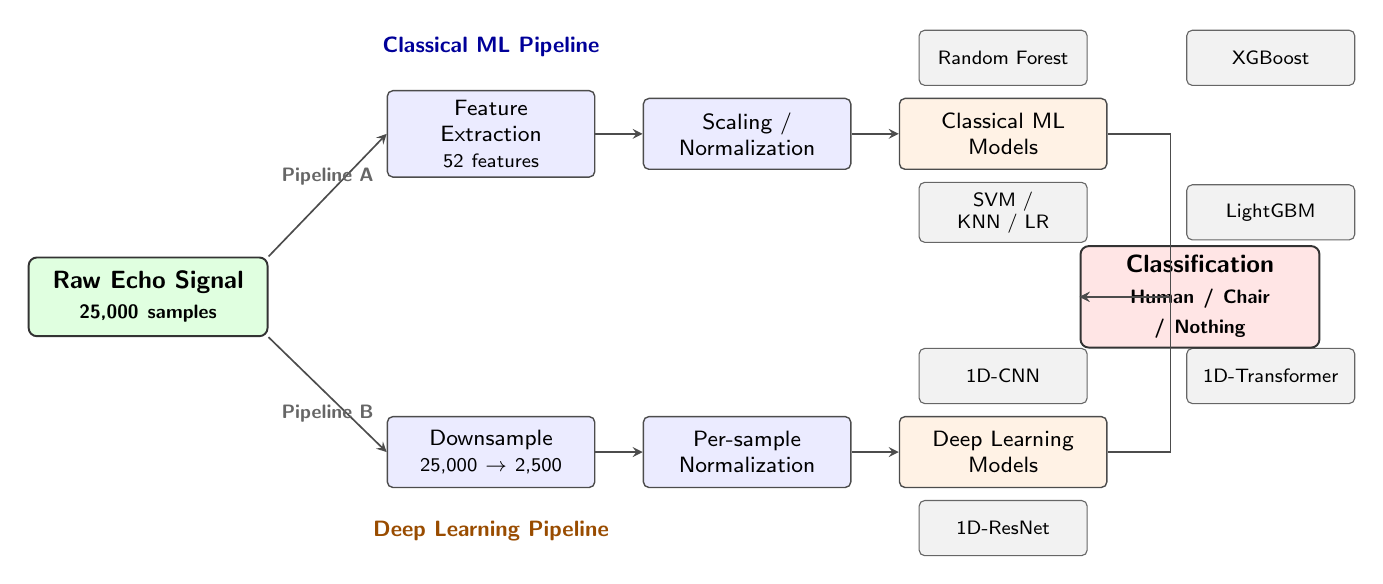
\begin{tikzpicture}[
    node distance=0.5cm and 0.8cm,
    block/.style={rectangle, draw=black!70, fill=blue!8, text width=2.4cm, minimum height=0.9cm, align=center, font=\footnotesize\sffamily, rounded corners=2pt, line width=0.5pt},
    bigblock/.style={rectangle, draw=black!70, fill=orange!10, text width=2.4cm, minimum height=0.9cm, align=center, font=\footnotesize\sffamily, rounded corners=2pt, line width=0.5pt},
    startblock/.style={rectangle, draw=black!80, fill=green!12, text width=2.8cm, minimum height=1cm, align=center, font=\small\sffamily\bfseries, rounded corners=3pt, line width=0.7pt},
    endblock/.style={rectangle, draw=black!80, fill=red!10, text width=2.8cm, minimum height=1cm, align=center, font=\small\sffamily\bfseries, rounded corners=3pt, line width=0.7pt},
    modelblock/.style={rectangle, draw=black!60, fill=gray!10, text width=1.9cm, minimum height=0.7cm, align=center, font=\scriptsize\sffamily, rounded corners=2pt},
    arrow/.style={->, >=stealth, line width=0.6pt, black!70},
    label/.style={font=\scriptsize\sffamily\bfseries, text=black!60},
]

% === INPUT ===
\node[startblock] (input) {Raw Echo Signal\\{\scriptsize 25,000 samples}};

% === TWO BRANCHES ===
% --- Classical ML Branch (top) ---
\node[block, above right=1.0cm and 1.5cm of input] (feat) {Feature\\Extraction\\{\scriptsize 52 features}};
\node[block, right=0.6cm of feat] (scale) {Scaling /\\Normalization};
\node[bigblock, right=0.6cm of scale] (classical) {Classical ML\\Models};

% Model sub-items for classical
\node[modelblock, above=0.15cm of classical, xshift=-0.0cm] (rf) {Random Forest};
\node[modelblock, below=0.15cm of classical, xshift=0.0cm] (svm) {SVM / KNN / LR};
\node[modelblock, right=0.05cm of rf, xshift=1.2cm] (xgb) {XGBoost};
\node[modelblock, right=0.05cm of svm, xshift=1.2cm] (lgb) {LightGBM};

% --- Deep Learning Branch (bottom) ---
\node[block, below right=1.0cm and 1.5cm of input] (ds) {Downsample\\{\scriptsize 25,000 $\to$ 2,500}};
\node[block, right=0.6cm of ds] (norm) {Per-sample\\Normalization};
\node[bigblock, right=0.6cm of norm] (deep) {Deep Learning\\Models};

% Model sub-items for deep learning
\node[modelblock, above=0.15cm of deep, xshift=0.0cm] (cnn) {1D-CNN};
\node[modelblock, below=0.15cm of deep, xshift=0.0cm] (resn) {1D-ResNet};
\node[modelblock, right=0.05cm of cnn, xshift=1.2cm] (trans) {1D-Transformer};

% === OUTPUT ===
\node[endblock, right=3.8cm of input, yshift=0.0cm, xshift=6.5cm] (output) {Classification\\{\scriptsize Human / Chair / Nothing}};

% === ARROWS ===
% Input to branches
\draw[arrow] (input.north east) -- (feat.west) node[midway, above, label] {Pipeline A};
\draw[arrow] (input.south east) -- (ds.west) node[midway, below, label] {Pipeline B};

% Classical branch
\draw[arrow] (feat) -- (scale);
\draw[arrow] (scale) -- (classical);

% Deep learning branch
\draw[arrow] (ds) -- (norm);
\draw[arrow] (norm) -- (deep);

% To output
\draw[arrow] (classical.east) -- ++(0.8,0) |- (output.west);
\draw[arrow] (deep.east) -- ++(0.8,0) |- (output.west);

% === BRANCH LABELS ===
\node[above=0.3cm of feat, font=\footnotesize\sffamily\bfseries, text=blue!60!black] {Classical ML Pipeline};
\node[below=0.3cm of ds, font=\footnotesize\sffamily\bfseries, text=orange!60!black] {Deep Learning Pipeline};

\end{tikzpicture}
}%
\caption{Functional block diagram of the two parallel classification pipelines. Pipeline~A extracts 52 handcrafted features from the raw signal and feeds them to classical ML models. Pipeline~B downsamples and normalizes the raw signal directly for end-to-end deep learning models. Both pipelines output a three-class prediction.}
\label{fig:block_diagram}
\end{figure}

\subsection{Preprocessing}

For the classical ML pipeline, the full 25{,}000-sample signal and the 17-element metadata vector were passed directly to the feature extraction stage described below. For the deep learning pipeline, we first downsampled each signal by a factor of 10---averaging every 10 consecutive samples---to reduce the input dimension from 25{,}000 to 2{,}500. Each downsampled signal was then independently normalized to zero mean and unit variance, ensuring that the network sees a consistent amplitude scale regardless of the raw ADC gain.

\subsection{Feature Engineering}

We extracted 52 numerical features from each signal, organized into six groups.

\subsubsection{Segmented Energy (28 features)}
The signal was split into 25 windows of 1{,}000 samples. For each window~$w_i$, the normalized energy fraction was computed as
\begin{equation}
    E_i = \frac{\sum_{n \in w_i} x[n]^2}{\sum_{n=0}^{N-1} x[n]^2},
    \label{eq:seg_energy}
\end{equation}
where $N = 25{,}000$. Three additional features captured the cumulative energy in three coarser regions: early (0--4\,ms), mid (4--8\,ms), and late (8--12.8\,ms).

\subsubsection{Global Statistics (8 features)}
Standard descriptors of the waveform shape: root-mean-square amplitude, standard deviation, peak positive and negative amplitudes, mean amplitude, mean absolute amplitude, and crest factor (ratio of peak to RMS).

\subsubsection{Peak and Echo Location (6 features)}
We smoothed the absolute-value envelope with a 500-sample moving average, applied a threshold at two standard deviations above the mean, and used peak detection to identify significant echoes. From the resulting peaks we recorded the count, the times of the first and last peak, the time of the overall amplitude maximum, and the temporal spread between the earliest and latest peak.

\subsubsection{Signal Shape (3 features)}
Skewness, kurtosis, and zero-crossing rate---three statistics that capture asymmetry, tail weight, and oscillatory character, respectively.

\subsubsection{Frequency Domain (5 features)}
From the magnitude spectrum obtained via FFT, we computed the total spectral energy, the dominant frequency, the spectral centroid
\begin{equation}
    f_c = \frac{\sum_{k} f_k \cdot |X[k]|}{\sum_{k} |X[k]|},
    \label{eq:centroid}
\end{equation}
the spectral bandwidth, and the energy concentrated in the 35--45\,kHz band around the sensor's 40\,kHz carrier.

\subsubsection{Metadata (2 features)}
The firmware-reported distance estimate (metadata column~11) and the onboard energy metric (column~17).

\subsection{Classical Machine Learning Models}

We evaluated six classifiers spanning different algorithmic families:

\begin{enumerate}
    \item \textbf{Random Forest} \cite{breiman2001}: 200 trees, maximum depth 20.
    \item \textbf{XGBoost} \cite{chen2016}: 200 boosting rounds, maximum depth 8, learning rate 0.1.
    \item \textbf{LightGBM} \cite{ke2017}: same hyperparameters as XGBoost, but using histogram-based leaf splitting for faster training.
    \item \textbf{SVM}: radial-basis-function kernel, $C=10$, $\gamma=\text{scale}$. Features were standardized to zero mean and unit variance.
    \item \textbf{KNN}: $k=5$ neighbors, with the same standardization.
    \item \textbf{Logistic Regression}: multinomial with $\ell_2$ penalty, maximum 1{,}000 iterations.
\end{enumerate}

\subsection{Deep Learning Architectures}

All three networks receive the downsampled 2{,}500-sample signal as a one-channel 1D input. None of them uses the handcrafted features.

\subsubsection{1D-CNN}
Four convolutional blocks, each consisting of a 1D convolution, batch normalization, ReLU, and max-pooling. The filter count doubles at each stage (32, 64, 128, 256) while the kernel size decreases (7, 5, 3, 3). After global average pooling, two dense layers (128 and 64 units) with dropout (0.3 and 0.2) feed a three-way softmax output. The network has 177{,}091 trainable parameters.

\subsubsection{1D-ResNet}
An initial strided convolution and max-pool reduce the temporal resolution, followed by four stages of two residual blocks each. Each block applies two convolution--batch-norm sequences and adds the input back to the output through a skip connection:
\begin{equation}
    \mathbf{y} = \mathcal{F}(\mathbf{x}) + \mathbf{x},
    \label{eq:resnet}
\end{equation}
where $\mathcal{F}$ denotes the stacked transformations within the block \cite{he2016}. Filter widths grow from 32 to 256 across the four stages. The classification head mirrors that of the CNN. Total parameters: 1{,}012{,}035.

\subsubsection{1D-Transformer}
Inspired by the Vision Transformer \cite{dosovitskiy2021}, we split the input into 50 non-overlapping patches of 50 samples each and project them to a 64-dimensional embedding space via a strided convolution. Learned positional encodings are added to preserve temporal ordering. Three Transformer blocks follow, each containing multi-head self-attention with four heads \cite{vaswani2017} and a two-layer feed-forward network (hidden size 128). The self-attention operation
\begin{equation}
    \mathrm{Attention}(Q,K,V) = \mathrm{softmax}\!\left(\frac{QK^\top}{\sqrt{d_k}}\right)V
    \label{eq:attention}
\end{equation}
allows every patch to attend to every other patch in a single step, making it straightforward for the model to compare, say, the early-time region (where Human echoes appear) with the late-time region (where floor echoes dominate). Global average pooling and two dense layers produce the final class probabilities. Total parameters: 269{,}635.

\subsection{Training Protocol}

To simulate a realistic deployment scenario where the model must generalize to measurements collected \emph{after} training, we used a temporal split rather than a random one: the first 80\% of each class (in recording order) served as training data, and the remaining 20\% formed the test set. Within the training partition, an 85/15 split provided a validation set for monitoring early stopping (patience 10--12 epochs) and learning-rate reduction on plateau. All deep learning models were optimized with Adam \cite{lecun2015}.

% ==============================================================
% IV. RESULTS
% ==============================================================
\section{Experimental Results}

\subsection{Classical Machine Learning}

Table~\ref{tab:classical_results} shows the test-set performance of the six classical models. Every model surpassed the 95\% accuracy target, with XGBoost and LightGBM sharing the top spot at 99.97\%. Inference times are negligible---under 0.05\,ms per sample in all cases.

\begin{table}[H]
\centering
\caption{Classical ML results on the temporal test set.}
\label{tab:classical_results}
\begin{tabular}{lccc}
\toprule
\textbf{Model} & \textbf{Accuracy (\%)} & \textbf{Train Time} & \textbf{Pred./Sample} \\
\midrule
XGBoost        & \textbf{99.97} & 1.8\,s & 0.01\,ms \\
LightGBM       & 99.97          & 1.5\,s & 0.01\,ms \\
Random Forest  & 99.93          & 8.2\,s & 0.03\,ms \\
KNN ($k$=5)    & 99.90          & ---    & 0.05\,ms \\
SVM (RBF)      & 99.83          & ---    & 0.02\,ms \\
Logistic Reg.  & 99.67          & ---    & 0.01\,ms \\
\bottomrule
\end{tabular}
\end{table}

XGBoost achieved 100\% accuracy on both Human and Chair, misclassifying only a single Nothing sample as Human across the entire 3{,}002-sample test set.

\subsection{Feature Importance}

Fig.~\ref{fig:feature_importance} ranks the 20 most informative features as determined by XGBoost's built-in importance metric. Peak amplitude and spectral bandwidth dominate, followed by the segmented energy in window~11 (corresponding to the 5--6\,ms region where chair reflections appear) and the firmware-reported distance. Together, features related to \emph{when} and \emph{how strongly} the echo arrives account for the vast majority of the model's discriminative power.

As a robustness check, we retrained the model after removing the two metadata-derived features (distance and energy metric). Accuracy dropped by only 0.04 percentage points, to 99.53\%. Training with just the top five features still yielded 95.24\%, indicating that the echo signal itself---independent of any firmware-computed summary---contains more than enough information for reliable classification.

\begin{figure}[H]
\centering
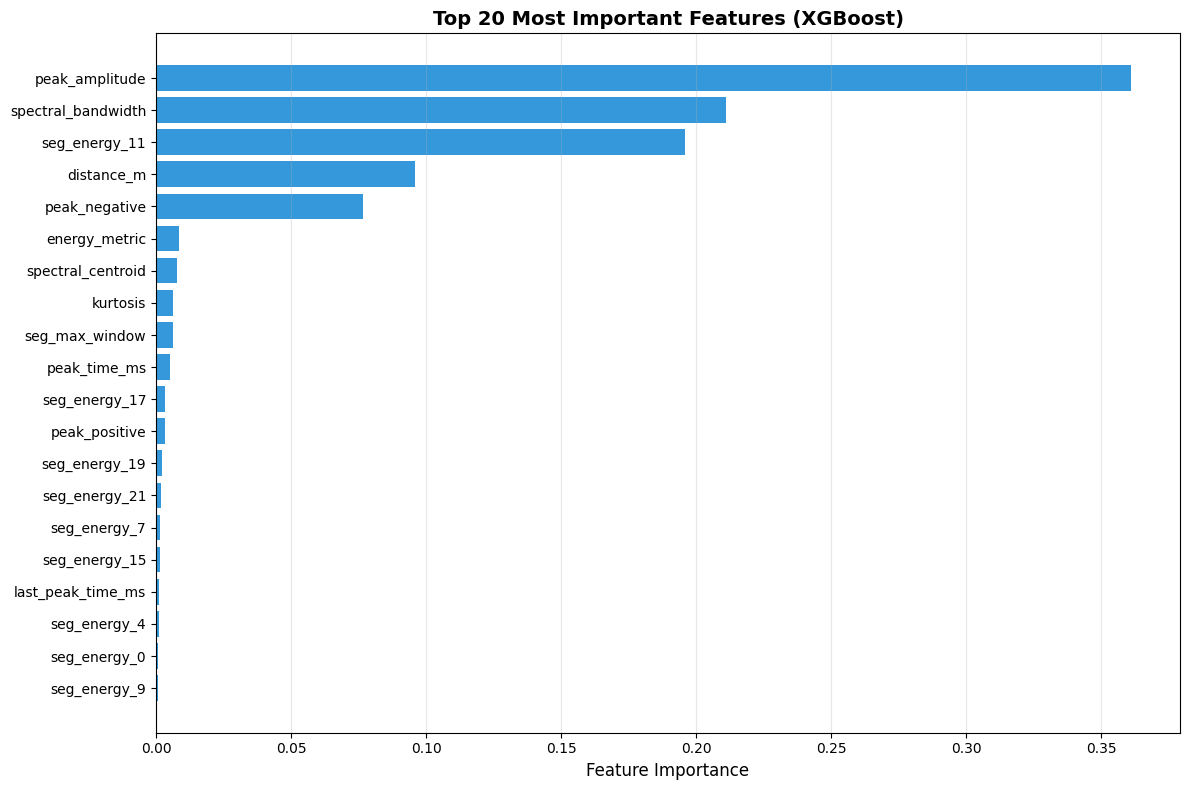
\includegraphics[width=\columnwidth]{fig_feature_importance.png}
\caption{Top 20 features by XGBoost importance. Peak amplitude, spectral bandwidth, and mid-range segmented energy dominate, reflecting the physical differences in how each object class reflects the ultrasonic pulse.}
\label{fig:feature_importance}
\end{figure}

\subsection{Deep Learning}

Table~\ref{tab:dl_results} compares the three neural network architectures. All three exceeded 99\% accuracy on the temporal test set, despite receiving only the raw downsampled waveform with no manually designed features.

\begin{table}[H]
\centering
\caption{Deep learning results on the temporal test set (raw signal input, no handcrafted features).}
\label{tab:dl_results}
\begin{tabular}{lccc}
\toprule
\textbf{Model} & \textbf{Accuracy (\%)} & \textbf{Pred./Sample} & \textbf{Parameters} \\
\midrule
1D-Transformer  & \textbf{99.53} & 1.75\,ms  & 269{,}635 \\
1D-CNN           & 99.33          & 0.89\,ms  & 177{,}091 \\
1D-ResNet        & 99.20          & 3.45\,ms  & 1{,}012{,}035 \\
\bottomrule
\end{tabular}
\end{table}

\subsection{Overfitting Validation}

We performed four complementary tests to verify that the high accuracy numbers reflect genuine signal differences rather than memorization.

\textbf{Temporal k-fold cross-validation.} The data were divided into five consecutive blocks per class, and each block served as the held-out test set in turn. The resulting mean accuracy was 99.94\% with a standard deviation of just 0.088\%, showing that performance is stable regardless of which temporal segment is withheld.

\textbf{Learning curves.} We trained on progressively larger fractions of the training set (5\%, 10\%, 20\%, \ldots, 100\%) and recorded both training and test accuracy. Even with only 5\% of the data ($\sim$600 samples), the test accuracy reached 99.87\%. The gap between training and test accuracy at full data was a mere 0.07\%, ruling out meaningful overfitting.

\textbf{Noise injection.} We added zero-mean Gaussian noise to the test features, scaling the noise standard deviation as a fraction of each feature's own standard deviation (5\%, 10\%, 20\%, \ldots, 200\%). Accuracy degraded smoothly rather than collapsing abruptly, which is the expected behavior of a model that has learned robust patterns rather than brittle memorized boundaries.

\textbf{Label shuffling.} As a sanity check, we randomly permuted the training labels and retrained a simplified Random Forest (depth~5) ten times. The mean test accuracy was approximately 33\%---indistinguishable from chance for a three-class problem---confirming that the real model's performance depends on the actual signal--label correspondence, not on spurious structure in the feature space.

\subsection{Head-to-Head: XGBoost vs.\ 1D-Transformer}

Table~\ref{tab:headtohead} distills the comparison between the best model from each paradigm. XGBoost holds a small accuracy edge (99.97\% vs.\ 99.53\%) and is roughly 175$\times$ faster at inference. On the other hand, the Transformer requires no feature engineering at all and---as discussed in Section~V---proved more dependable when deployed on live sensor data.

\begin{table}[H]
\centering
\caption{Head-to-head comparison of the best classical ML model and the best deep learning model.}
\label{tab:headtohead}
\begin{tabular}{lcc}
\toprule
                          & \textbf{XGBoost}     & \textbf{1D-Transformer} \\
\midrule
Approach                  & Classical ML          & Deep Learning \\
Input                     & 52 features           & Raw signal (2{,}500 pts) \\
Overall Accuracy          & \textbf{99.97\%}      & 99.53\% \\
Human Accuracy            & 100.00\%              & 98.80\% \\
Chair Accuracy            & 100.00\%              & 100.00\% \\
Nothing Accuracy          & 99.90\%               & 99.80\% \\
Inference / Sample        & \textbf{0.01\,ms}     & 1.75\,ms \\
Trainable Parameters      & ---                   & 269{,}635 \\
Feature Engineering       & Required              & \textbf{Not required} \\
\bottomrule
\end{tabular}
\end{table}

Figs.~\ref{fig:cm_xgboost} and \ref{fig:cm_transformer} show the confusion matrices for both models. XGBoost commits only a single misclassification (one Nothing sample predicted as Human). The Transformer makes 14 errors in total, most of which involve Human samples predicted as Chair---a confusion that is physically plausible given that the human body occasionally produces a focused reflection resembling a hard-surface echo.

\begin{figure}[H]
\centering
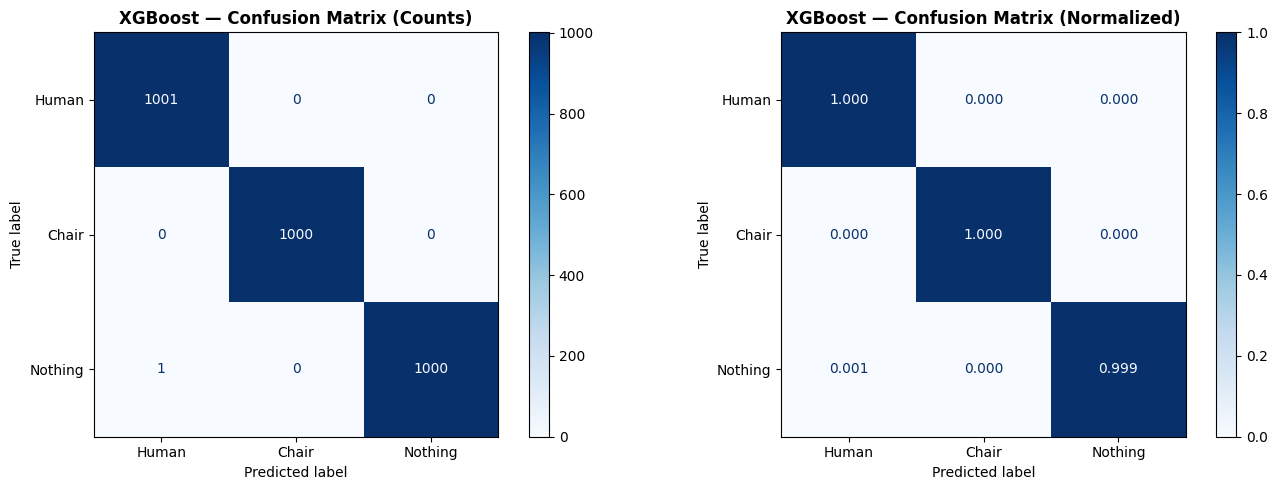
\includegraphics[width=\columnwidth]{fig_confusion_matrix.png}
\caption{Confusion matrix for XGBoost (best classical ML). Left: absolute counts; right: row-normalized proportions. Only one Nothing sample is misclassified.}
\label{fig:cm_xgboost}
\end{figure}

\begin{figure}[H]
\centering
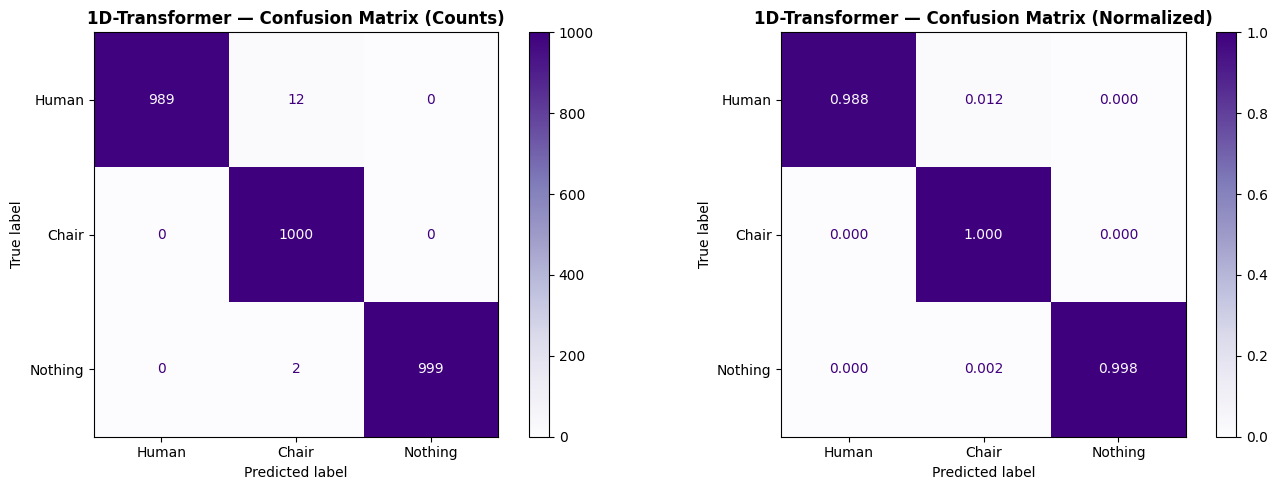
\includegraphics[width=\columnwidth]{fig_transformer_confusion.png}
\caption{Confusion matrix for the 1D-Transformer (best deep learning). Chair is classified perfectly; a small number of Human samples are confused with Chair.}
\label{fig:cm_transformer}
\end{figure}

\subsection{Real-Time Deployment}

To move beyond offline evaluation, we built a desktop application in PyQt6 that connects to the Red Pitaya board over UDP and classifies each incoming echo signal in real time. The application runs all three deep learning models---Transformer, ResNet, and CNN---in parallel on every received waveform and displays the per-model prediction, confidence score, and a majority-vote consensus. Figs.~\ref{fig:rt_human},~\ref{fig:rt_chair}, and~\ref{fig:rt_nothing} show representative screenshots for each of the three object classes during live operation.

\begin{figure}[H]
\centering
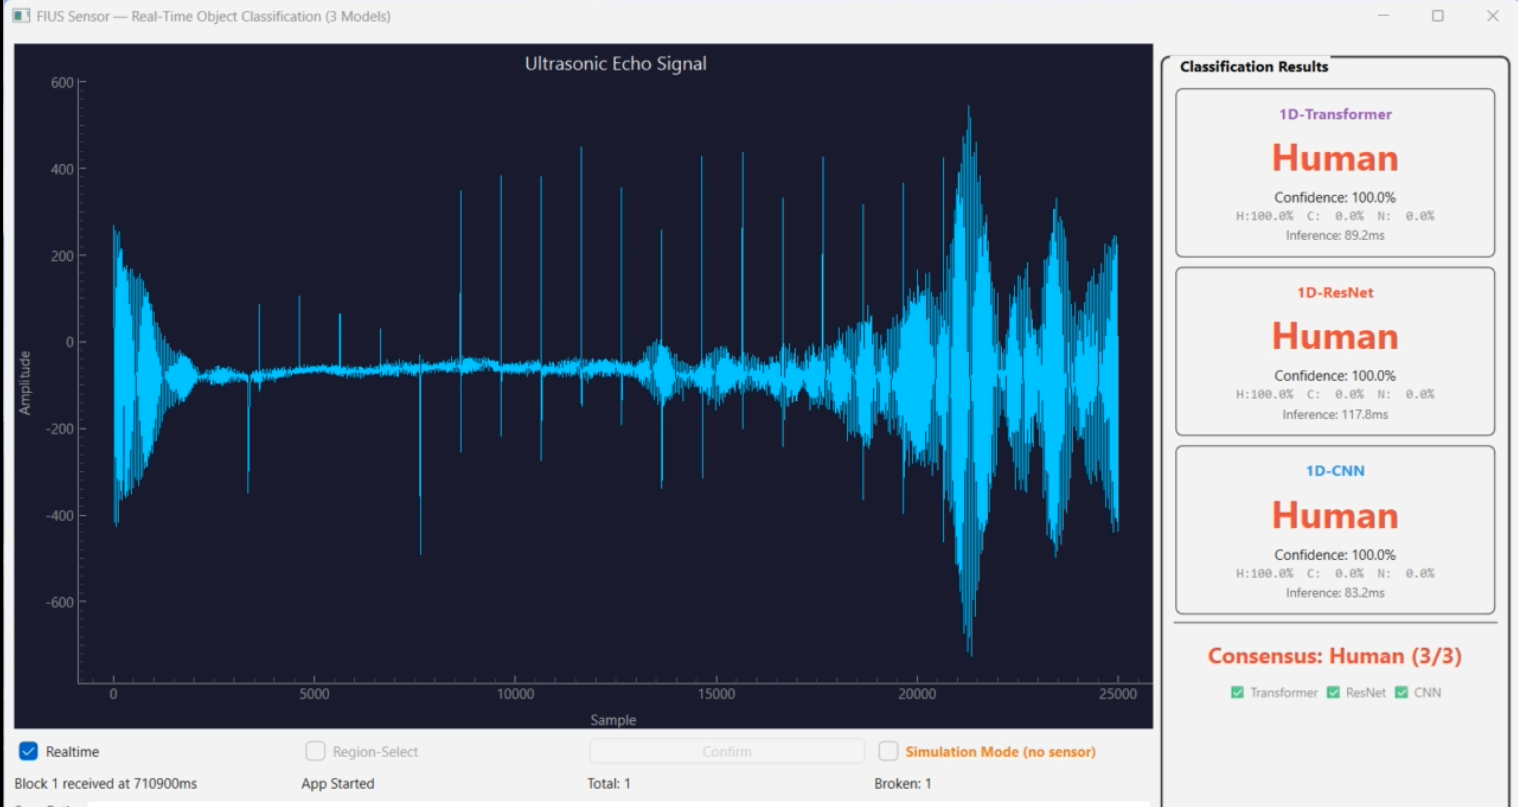
\includegraphics[width=\columnwidth]{fig_real_time_human_classification.png}
\caption{Real-time Human detection: all three models agree with 100\% confidence. Consensus: Human (3/3).}
\label{fig:rt_human}
\end{figure}

\begin{figure}[H]
\centering
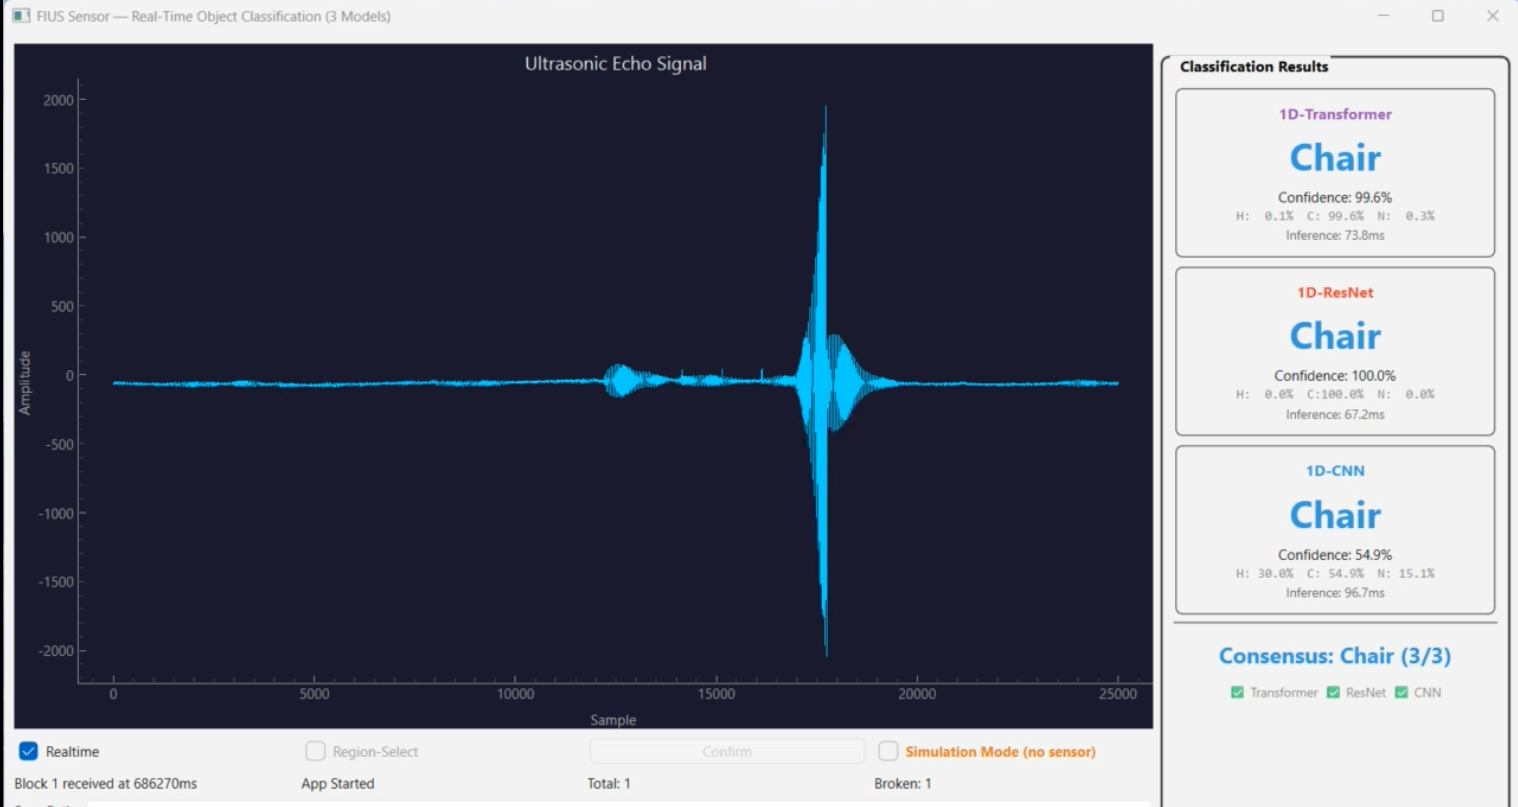
\includegraphics[width=\columnwidth]{fig_real_time_chair_classification.png}
\caption{Real-time Chair detection: Transformer 99.6\%, ResNet 100\%, CNN 54.9\%. Consensus: Chair (3/3).}
\label{fig:rt_chair}
\end{figure}

\begin{figure}[H]
\centering
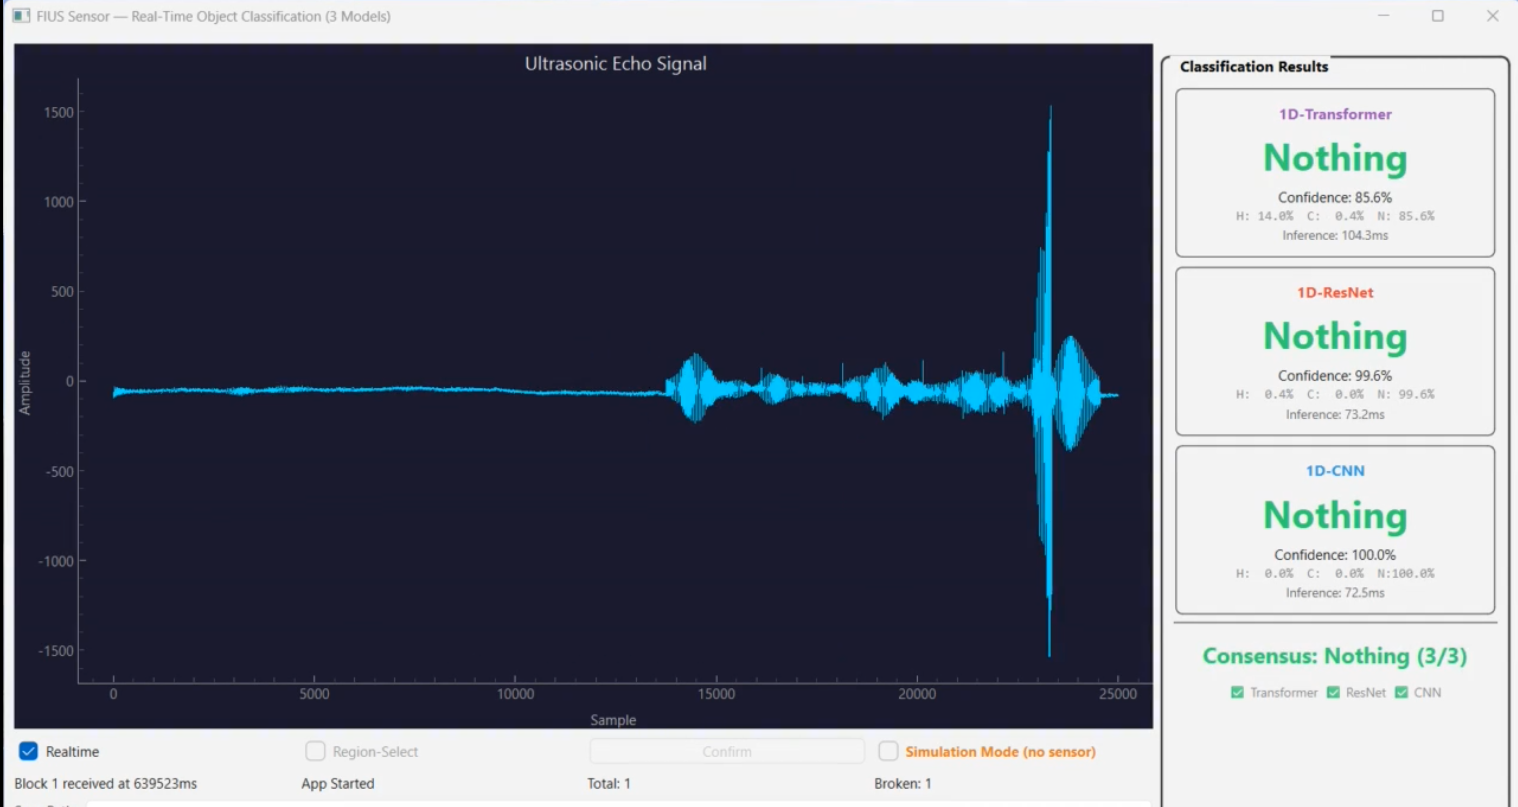
\includegraphics[width=\columnwidth]{fig_real_time_nothing_classification.png}
\caption{Real-time Nothing detection: CNN 100\%, ResNet 99.6\%, Transformer 85.6\%. Consensus: Nothing (3/3).}
\label{fig:rt_nothing}
\end{figure}

Several patterns emerged during live testing. Human was the most reliably detected class: the Transformer and ResNet both identified it with 100\% confidence in nearly every reading, and the CNN agreed in most cases. For Chair, the ResNet performed most consistently (typically 100\% confidence), with the Transformer close behind ($\sim$99\%), while the CNN was noticeably less certain ($\sim$55\%), occasionally splitting its probability mass between Chair and Human. For Nothing, the roles partially reversed: the CNN was often the most confident (up to 100\%), while the Transformer sometimes assigned non-trivial probability to Human.

Table~\ref{tab:realtime_summary} summarizes these observations. Across all three classes, the majority-vote consensus produced the correct label in approximately 70--80\% of live readings. Most of the remaining cases involved momentary disagreements among models rather than consistent misclassification, and no class was systematically confused with another.

\begin{table}[H]
\centering
\caption{Qualitative summary of real-time model behavior on live sensor data.}
\label{tab:realtime_summary}
\begin{tabular}{lccc}
\toprule
\textbf{Class} & \textbf{Transformer} & \textbf{ResNet} & \textbf{CNN} \\
\midrule
Human   & Strong   & Strong    & Strong \\
Chair   & Strong   & Strongest & Uncertain \\
Nothing & Moderate & Strong    & Strongest \\
\bottomrule
\end{tabular}
\end{table}

Inference latency on the host PC ranged from 67 to 118\,ms per model per signal, depending on the architecture and system load. While this is slower than the sub-2\,ms offline numbers (which excluded data transfer and Python overhead), it remains fast enough for the application's target update rate of roughly one classification per second.

The gap between offline accuracy ($>$99\%) and live accuracy ($\sim$70--80\%) can be attributed to several factors. The live signal passes through a different data path (UDP packets assembled from multiple blocks) than the CSV files used for training, introducing occasional packet-timing artifacts. Environmental conditions in the lab---air currents, slight sensor vibrations, ambient noise---add variability not present in the training set. The consensus mechanism partly compensates for these effects: even when individual models disagree, the majority vote tends to land on the correct class.
% ==============================================================
% V. DISCUSSION
% ==============================================================
\section{Discussion}

\subsection{Classical ML vs.\ Deep Learning}

On paper, XGBoost outperforms the Transformer by a slim margin (99.97\% vs.\ 99.53\%). In practice, however, the picture is more nuanced. The classical ML pipeline depends on an intermediate feature extraction step that must reproduce \emph{exactly} the same computation used during training. When we first attempted to run XGBoost on live sensor data, subtle differences in how the real-time application assembled the signal array---compared to how the CSV training files were parsed---caused the extracted features to shift just enough to degrade predictions. The deep learning models, by contrast, accept the raw waveform directly and proved immediately functional on live data without any such calibration issues. This experience suggests that, for embedded or field-deployed systems where data formats may evolve over time, end-to-end deep learning pipelines offer a practical robustness advantage that purely numerical accuracy comparisons do not capture.

\subsection{Why Architecture Matters}

The three deep learning models illustrate how architectural choices interact with signal structure. The 1D-CNN processes the waveform through a stack of local convolution--pooling stages. By the time the network's deepest layers see the signal, the temporal resolution has been reduced several-fold, making it hard to simultaneously attend to the 6\,ms Chair echo and the 10.5\,ms floor echo---regions separated by thousands of raw samples. This limitation manifested early in development as a near-random Chair--Nothing confusion.

The ResNet addresses the depth problem through skip connections that let gradient and information flow across many layers without attenuation. In our experiments, it matched or exceeded the CNN on every class and was particularly strong on Chair, where it regularly achieved 100\% confidence during live inference.

The Transformer takes a fundamentally different approach. By computing pairwise attention scores between all 50 signal patches, it can directly compare the early, mid, and late portions of the waveform in a single computation. This makes it naturally suited to a classification task whose answer depends on \emph{where} the echo energy is concentrated along the time axis. Its main weakness---a tendency to assign non-trivial probability to Human when processing Nothing signals in real time---may reflect the fact that both classes produce some energy in the late-time region, and the live signal is noisier than the training data.

\subsection{Physical Interpretability}

The results are consistent with basic ultrasonic physics. Soft tissue absorbs and scatters 40\,kHz sound waves, producing a broad, low-amplitude echo. A hard surface reflects them specularly, generating a short, high-amplitude pulse at a delay proportional to the object's distance. An unobstructed floor produces only a single strong return at the maximum range. The feature importance plot (Fig.~\ref{fig:feature_importance}) confirms that the model relies on precisely these physical cues: peak amplitude (how strong?), spectral bandwidth (how spread out?), and segmented energy in the mid-time windows (is there a chair-distance echo?). The classification is not an opaque statistical trick but a direct reflection of material-dependent acoustic behavior.

% ==============================================================
% VI. CONCLUSION
% ==============================================================
\section{Conclusion}

We set out to determine whether a single 40\,kHz ultrasonic sensor can distinguish a human body from an office chair and from an empty floor, and the answer is a clear yes. Both classical ML (XGBoost, 99.97\%) and deep learning (1D-Transformer, 99.53\%) exceeded the 95\% accuracy target by a wide margin on temporally separated test data. Four independent overfitting checks---temporal cross-validation, learning curves, noise injection, and label shuffling---confirmed that the models learned genuine physical patterns rather than dataset artifacts.

Deploying the models on live sensor data introduced new challenges: data-path differences, environmental noise, and packet-timing variability reduced effective accuracy to an estimated 70--80\%. A majority-vote ensemble across three deep learning architectures mitigated much of this gap and provided correct classifications for all three classes in real time. Among the individual models, the Transformer and ResNet were the most reliable, with complementary strengths---the Transformer excelling on Human, the ResNet on Chair, and the CNN on Nothing.

Several directions remain open for future work. Expanding the class set to include additional objects (e.g., different furniture types, pets, or multiple people) would test the limits of the approach. Varying the sensor height and angle would assess geometric generalization. On the deployment side, converting the models to TensorFlow Lite and running them on edge hardware (e.g., a Raspberry Pi or the Red Pitaya itself) would eliminate the host-PC dependency and bring the system closer to a standalone embedded product.

% ==============================================================
% REFERENCES
% ==============================================================
\begin{thebibliography}{00}

\bibitem{carullo2001}
A.~Carullo and M.~Parvis, ``An ultrasonic sensor for distance measurement in automotive applications,'' \textit{IEEE Sensors Journal}, vol.~1, no.~2, pp.~143--147, Aug. 2001.

\bibitem{he2016}
K.~He, X.~Zhang, S.~Ren, and J.~Sun, ``Deep residual learning for image recognition,'' in \textit{Proc. IEEE Conf. Computer Vision and Pattern Recognition (CVPR)}, 2016, pp.~770--778.

\bibitem{dosovitskiy2021}
A.~Dosovitskiy \textit{et al.}, ``An image is worth 16x16 words: Transformers for image recognition at scale,'' in \textit{Proc. Int. Conf. Learning Representations (ICLR)}, 2021.

\bibitem{breiman2001}
L.~Breiman, ``Random forests,'' \textit{Machine Learning}, vol.~45, no.~1, pp.~5--32, 2001.

\bibitem{chen2016}
T.~Chen and C.~Guestrin, ``XGBoost: A scalable tree boosting system,'' in \textit{Proc. 22nd ACM SIGKDD Int. Conf. Knowledge Discovery and Data Mining}, 2016, pp.~785--794.

\bibitem{ke2017}
G.~Ke \textit{et al.}, ``LightGBM: A highly efficient gradient boosting decision tree,'' in \textit{Advances in Neural Information Processing Systems}, vol.~30, 2017.

\bibitem{vaswani2017}
A.~Vaswani \textit{et al.}, ``Attention is all you need,'' in \textit{Advances in Neural Information Processing Systems}, vol.~30, 2017.

\bibitem{lecun2015}
Y.~LeCun, Y.~Bengio, and G.~Hinton, ``Deep learning,'' \textit{Nature}, vol.~521, no.~7553, pp.~436--444, 2015.

\bibitem{sklearn}
F.~Pedregosa \textit{et al.}, ``Scikit-learn: Machine learning in Python,'' \textit{Journal of Machine Learning Research}, vol.~12, pp.~2825--2830, 2011.

\bibitem{tensorflow}
M.~Abadi \textit{et al.}, ``TensorFlow: A system for large-scale machine learning,'' in \textit{Proc. 12th USENIX Symp. Operating Systems Design and Implementation (OSDI)}, 2016, pp.~265--283.

\end{thebibliography}

\end{document}